% This must be in the first 5 lines to tell arXiv to use pdfLaTeX, which is strongly recommended.
\pdfoutput=1
% In particular, the hyperref package requires pdfLaTeX in order to break URLs across lines.

\documentclass[11pt]{article}

% Change "review" to "final" to generate the final (sometimes called camera-ready) version.
% Change to "preprint" to generate a non-anonymous version with page numbers.
% \usepackage[review]{acl}
\usepackage[preprint]{acl}

% Standard package includes
\usepackage{times}
\usepackage{latexsym}

% For proper rendering and hyphenation of words containing Latin characters (including in bib files)
\usepackage[T1]{fontenc}
% For Vietnamese characters
% \usepackage[T5]{fontenc}
% See https://www.latex-project.org/help/documentation/encguide.pdf for other character sets

% This assumes your files are encoded as UTF8
\usepackage[utf8]{inputenc}

% This is not strictly necessary, and may be commented out,
% but it will improve the layout of the manuscript,
% and will typically save some space.
\usepackage{microtype}

% This is also not strictly necessary, and may be commented out.
% However, it will improve the aesthetics of text in
% the typewriter font.
\usepackage{inconsolata}

%Including images in your LaTeX document requires adding
%additional package(s)
\usepackage{graphicx}

% Jack!
% \usepackage{amsmath}

% If the title and author information does not fit in the area allocated, uncomment the following
%
%\setlength\titlebox{<dim>}
%
% and set <dim> to something 5cm or larger.

\title{Modern Byte Pair Tokenizers are Zipfian}

% Author information can be set in various styles:
% For several authors from the same institution:
% \author{Author 1 \and ... \and Author n \\
%         Address line \\ ... \\ Address line}
% if the names do not fit well on one line use
%         Author 1 \\ {\bf Author 2} \\ ... \\ {\bf Author n} \\
% For authors from different institutions:
% \author{Author 1 \\ Address line \\  ... \\ Address line
%         \And  ... \And
%         Author n \\ Address line \\ ... \\ Address line}
% To start a separate ``row'' of authors use \AND, as in
% \author{Author 1 \\ Address line \\  ... \\ Address line
%         \AND
%         Author 2 \\ Address line \\ ... \\ Address line \And
%         Author 3 \\ Address line \\ ... \\ Address line}

\author{Jack Hanke \\
  Northwestern University \\
  \And
  Daniel Plotkin \\
  Northwestern University \\
  \And
  Nicole Birova \\
  Northwestern University}

%\author{
%  \textbf{First Author\textsuperscript{1}},
%  \textbf{Second Author\textsuperscript{1,2}},
%  \textbf{Third T. Author\textsuperscript{1}},
%  \textbf{Fourth Author\textsuperscript{1}},
%\\
%  \textbf{Fifth Author\textsuperscript{1,2}},
%  \textbf{Sixth Author\textsuperscript{1}},
%  \textbf{Seventh Author\textsuperscript{1}},
%  \textbf{Eighth Author \textsuperscript{1,2,3,4}},
%\\
%  \textbf{Ninth Author\textsuperscript{1}},
%  \textbf{Tenth Author\textsuperscript{1}},
%  \textbf{Eleventh E. Author\textsuperscript{1,2,3,4,5}},
%  \textbf{Twelfth Author\textsuperscript{1}},
%\\
%  \textbf{Thirteenth Author\textsuperscript{3}},
%  \textbf{Fourteenth F. Author\textsuperscript{2,4}},
%  \textbf{Fifteenth Author\textsuperscript{1}},
%  \textbf{Sixteenth Author\textsuperscript{1}},
%\\
%  \textbf{Seventeenth S. Author\textsuperscript{4,5}},
%  \textbf{Eighteenth Author\textsuperscript{3,4}},
%  \textbf{Nineteenth N. Author\textsuperscript{2,5}},
%  \textbf{Twentieth Author\textsuperscript{1}}
%\\
%\\
%  \textsuperscript{1}Affiliation 1,
%  \textsuperscript{2}Affiliation 2,
%  \textsuperscript{3}Affiliation 3,
%  \textsuperscript{4}Affiliation 4,
%  \textsuperscript{5}Affiliation 5
%\\
%  \small{
%    \textbf{Correspondence:} \href{mailto:email@domain}{email@domain}
%  }
%}

\begin{document}
\maketitle
\begin{abstract}
A majority of large language models ingest word fragments called \textit{tokens} produced by a data compression algorithm known as byte pair encoding. This algorithm groups high-frequency letter pairings in natural language into individual units. A natural question is whether the tokens produced by this pairing process deviate significantly from the source language's frequency distribution. Zipf famously showed that many natural language's frequency distribution follows a power law, commonly known as Zipf's Law. We examine two modern tokenizer's adherence to Zipf's law at the token level. We demonstrate that these tokenizers are Zipfian on two corpuses, and speculate as to why this is.
\end{abstract}

\section{Introduction}

George Zipf in his hallmark \textit{The Psycho-Biology of Language} \cite{Zip35} introduced the remarkable trend that the word frequencies in many human languages exhibit the same power law distribution. Specifically, Zipf said that the frequency  that a word appears in some large corpus is proportional to the word's frequency rank. Mathematically, Zipf's laws states

\begin{equation}
    \mbox{word frequency} \propto \frac{1}{\mbox{word rank}}.
\end{equation}

A more descriptive model of word frequency that is more commonly referenced in linguistics literature is the Zipf-Mandelbrot distribution

\begin{equation}
    \mbox{word frequency} \propto \frac{1}{(\mbox{word rank} + b)^a}.
    \label{eq:zipfmandelbrot}
\end{equation}

where $a,b$ are fitted parameters. We say a distribution that follows the trend in Equation \ref{eq:zipfmandelbrot} with $a \approx 1$ is \textit{Zipf distributed}, or simply \textit{Zipfian}.

The accuracy of the trend in Equation \ref{eq:zipfmandelbrot} has been examined in $10^8$ English words in \cite{cancho2000}, over 50 languages in \cite{yu2018zipfslaw50languages}, and written-versus-spoken corpuses in \cite{lin2015scalinglawshumanspeech}. Each of these studies demonstrate that Zipf's law is generally exhibitted for common and somewhat-uncommon words, but rare words (words with high rank) appear less frequently than predicted. This deviation is shown to be statistically significant, and appears as two trendlines in the log-log plot. In English corpuses, this transition is found around the $10^5$\textit{-th} ranked word.\footnote{Some of these studies also find that extremely common words appear slighly more commonly than the Zipfian prediction.} The authors further explore the linguistic relavence and universality of these multiple regimes of words. 

Nearly a century after Zipf's discovery, large language models (LLMs) generate text comparable to human communication. However, unlike humans, LLMs digest text using a fixed vocabulary of word fragments called \textit{tokens}. The mapping between natural language and tokens is most commonly computed using the \textit{byte pair encoding algorithm} \cite{bpegage} over some large training corpus. Byte pair encoding identifies the most frequent pair of letters, and creates a new token in the "token vocabulary" to replace that pair. Iterating this procedure until some fixed vocabulary size is reached creates the vocabulary of tokens. Finally, any sequence that does not map to one of the derived tokens is labelled with the \texttt{<unk>} token, standing for unknown.

When considering these ideas in tandem, a natural question arises: given a corpus that appears Zipfian, how does the tokenization process affect this trend?

\section{Methods}

To explore this question, we choose two modern tokenizers to analyze. We choose the tokenizer for the RoBERTa language model \cite{liu2019robertarobustlyoptimizedbert}, as the training data is publicly known. This allows us to conduct frequency analyses on corpuses that are on and off-distribution for the tokenizer. We also choose to compare our results with the tokenizer for the GPT-4 language model \cite{openai2024gpt4technicalreport} as a representative of an industry-grade tokenizer. 

We choose two corpuses based on RoBERTa's training data. We choose the 4.4GB bookscorpus dataset \cite{zhu2015aligningbooksmoviesstorylike}, as RoBERTa's tokenizer was trained (in-part) on this corpus. For our off-distribution corpus, we choose the 5.6GBtying MiniPile dataset \cite{kaddour2023minipilechallengedataefficientlanguage}, which was released after the RoBERTa model was released. Note that it is likely that the GPT-4 tokenizer was trained (in-part) on both of these corpuses.

We compute the word and token frequency for both tokenizers on each corpus, where we define a word as anything separated by a space. We then compute the data's Kolmogorov-Smirnov goodness-of-fit statistic for the Zipf distribution, and compare to that for an exponential and log-normal distribution. We do not remove any tokens from consideration unless otherwise stated.

\section{Results}

We find that token vocabularies are remarkably Zipfian, excluding extremely rare tokens. This holds true for both tokenizers and both corpuses studied, including out-of-distribution text. In the log-log plots in Figure \ref{fig:experiments}, we show sharp declines from the Zipfian trend only for the final few tokens in the RoBERTa tokenizer for both corpuses and the GPT-4 tokenizer for the MiniPile corpus. However, the GPT-4 tokenizer trend on the bookscorpus seems to deviate more dramatically, similar to the multiple regime studies.

\begin{figure}[t]
  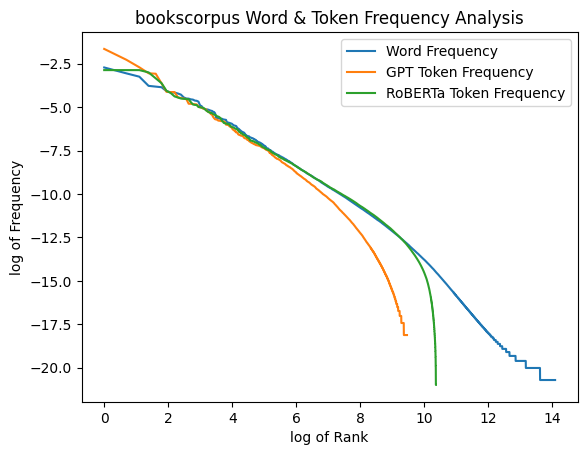
\includegraphics[width=\columnwidth]{../visualizations/bookscorpusfreq.png}
  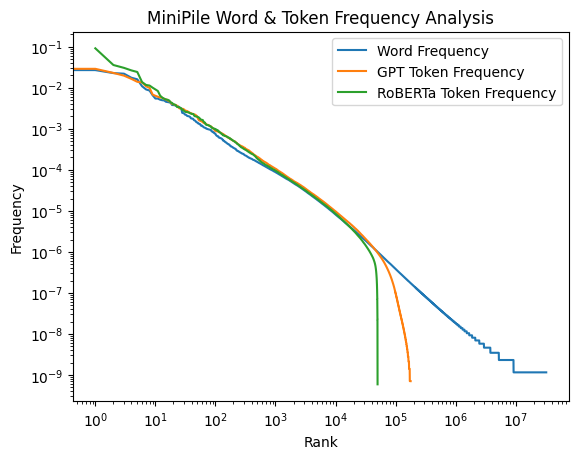
\includegraphics[width=\columnwidth]{../visualizations/minipilecorpusfreq.png}
  \caption{Log-log plots of word \& token rank vs word \& token frequency}
  \label{fig:experiments}
\end{figure}

The lowest rank words and tokens for each tokenizer and each corpus, including control tokens and punctuation, are summarized in Table \ref{tbl:token ranks}.

\begin{table}
    \centering
    \begin{tabular}{|c|c|c|c|c|c|c|}
        \hline
        \textbf{Rank} & \multicolumn{2}{c|}{\textbf{Words}} & \multicolumn{2}{c|}{\textbf{RoBERTa}} & \multicolumn{2}{c|}{\textbf{GPT-4}}  \\
        \hline
        1 & . & the & <s> & ␣ & `` & , \\
        \hline
        2 & , & of & \textbackslash n & \textbackslash n & i & ␣the \\
        \hline
        3 & the & and & <\textbackslash s> & . & he & . \\
        \hline
    \end{tabular}
    \caption{Summary of most common words \& tokens for each corpus, where the left subcolumn is bookscorpus and the right subcolumn MiniPile, including control tokens and punctuation}
    \label{tbl:token ranks}
\end{table}

\begin{table}
    \centering
    \begin{tabular}{|c|c|c|c|c|c|c|}
        \hline
        \textbf{Rank} & \multicolumn{2}{c|}{\textbf{Words}} & \multicolumn{2}{c|}{\textbf{RoBERTa}} & \multicolumn{2}{c|}{\textbf{GPT-4}}  \\
        \hline
        1 & the & the & the & the & i & the \\
        \hline
        2 & to & of & to & of & he & of \\
        \hline
        3 & i & and & and & and & she & and \\
        \hline
    \end{tabular}
    \caption{Summary of most common words \& tokens for each corpus, where the left subcolumn is bookscorpus and the right subcolumn MiniPile, \textit{not} including control tokens and punctuation}
    \label{tbl:token ranks no control}
\end{table}

The Kolmogorov-Smirnov test statistics for each considered distribution are summarized in Table \ref{tbl:kstest}.

\begin{table}
    \centering
    \begin{tabular}{|c|c|c|c|c|c|c|}
        \hline
        \textbf{Distribution} & \multicolumn{2}{c|}{\textbf{Words}} & \multicolumn{2}{c|}{\textbf{RoBERTa}} & \multicolumn{2}{c|}{\textbf{GPT-4}}  \\
        \hline
        Zipf &  &  &  &  &  &  \\
        \hline
        Exponential & 0.874 & 0.808 & 0.580 & 0.482 & 0.718 & 0.563 \\
        \hline
        log-normal & 0.379 & 0.451 & 0.032 & 0.050 & 0.397 & 0.283 \\
        \hline
    \end{tabular}
    \caption{Kolmogorov-Smirnov test statistics for distribution fit, where the left subcolumn is bookscorpus and the right subcolumn MiniPile}
    \label{tbl:kstest}
\end{table}


\section{Conclusions}

Despite 


\section{Future Work}

TODO

How do token vocabularies differ from english vocabularies? Fixed vocabulary size, catchall token, functional tokens

% Bibliography entries for the entire Anthology, followed by custom entries
%\bibliography{anthology,custom}
% Custom bibliography entries only
\bibliography{custom}

% \appendix

% \section{Example Appendix}
% \label{sec:appendix}

% This is an appendix.

\end{document}